\documentclass[12pt,spanish,letterpaper,color]{uchile}
\usepackage{ucs}
\usepackage[utf8x]{inputenc}
\usepackage[spanish]{babel}
\PrerenderUnicode{áéíóúÁÉÍÓÚüÜ}
%%%%%%%%%%%%%%%%%%%%%%
%% Para macros propias
\usepackage{xspace}

%move to class?
%%usa punto en vez de coma en las ecuaciones con decimales, tiene que ir despues de babel
\decimalpoint
%%%%%%%%%%%%%%%%%%%%%%
%% Mathematical packages
\usepackage{amsmath}
\usepackage{amsthm}
\usepackage{amssymb}

%move to class?
%%  paquete para setear los margenes, verificar
\usepackage[right=2cm,left=3cm,top=2cm,bottom=2cm,headsep=0cm,footskip=1cm]{geometry}
%\usepackage{anysize}
%\papersize{27.94cm}{21.59cm}
%\marginsize{3.0cm}{2.0cm}{2.0cm}{2.0cm}


%move to class?
%% paquete para insertar links en pdf
%colorlinks=true, resalta los links con colores
\usepackage[pdftex,pdfborderstyle={/S/U/W 0}, 
pdftitle={Memoria}, 
pdfauthor={Felipe Lema}, 
pdfsubject={Emulación}, pdfkeywords={p2p, kaillera, emulación},
pdfcreator={Felipe Lema}]{hyperref}

%%%%%%%%%%%%%%%%%%%%%%
%% Cite Package
%% must go after hyperref
%% debe ir depues de hyperref
\usepackage{cite}

%%%%%%%%%%%%%%%%%%%%%%
%% Numprint Pacakge
%% allows to print number with automatic thousand separator and decimal separator
%% Ejxamples: \numprint{2006.3}-> 2.006,3 \numprint{20009}-> 20.009
%% permite escribir numeros con separador de miles y con separador decimal. 
%% Ejemplos: \numprint{2006.3}-> 2.006,3 \numprint{20009}-> 20.009
\usepackage[autolanguage]{numprint}
\npthousandsep{.}\npdecimalsign{,}

%\renewcommand{\bibliographyname}{Bibliografía u otro nombre}
%%%%%%%%%%%%%%%%%%%%%%
%% Listings Package
%% Printing program/source code (C++ code)
%% Imprime código fuente/ de programa (código C++)
\usepackage{listings}
\usepackage{color}
\definecolor{gray97}{gray}{.97}
\definecolor{gray75}{gray}{.75}
\definecolor{gray45}{gray}{.45}

\lstset{ frame=Ltb,
     framerule=0pt,
     aboveskip=0.5cm,
     framextopmargin=3pt,
     framexbottommargin=3pt,
     framexleftmargin=0.4cm,
     framesep=0pt,
     rulesep=.4pt,
     backgroundcolor=\color{gray97},
     rulesepcolor=\color{black},
     %
     stringstyle=\ttfamily,
     showstringspaces = false,
     basicstyle={\ttfamily\small},
     commentstyle=\color{gray45},
     keywordstyle=\bfseries,
     %
     numbers=left,
     numbersep=15pt,
     numberstyle=\tiny,
     numberfirstline = false,
     breaklines=true,
     %
     float,
     language=C++,
     columns=fixed,
     escapeinside={//*}{\^^M}, %labels
     tabsize=2
   }
\renewcommand{\lstlistlistingname}{Códigos}
\renewcommand{\lstlistingname}{Código}

%%%%%%%%%%%%%%%%%%%%%%
%% Algorithms Package
%% Printing pseudocode
%% Imprime pseudo-código
\usepackage{algorithmic}


%%%%%%%%%%%%%%%%%%%%%%
%% clrscode3e Package
%% Typeset pseudo-code "Intro to Algorithms" style
%% Formatea pseudo-código al estilo de "Introducción a Algoritmos"
\usepackage{clrscode3e}

%%%%%%%%%%%%%%%%%%%%%%
%% subfig Package
%% to have subfigures within figures, or subtables within table floats
\usepackage{subfig}

\begin{document}
%%%%%%%%%%%%%%%%%%%%
%macros
%%%%%%%%%%%%%%%%%%%%
\newcommand{\kai}{\textit{Kaillera}\xspace}
\newcommand{\fba}{\texttt{fba}\xspace}


%%%%%%%%%%%%%%%%%%%%
%Definicion de variables de la portada
%%%%%%%%%%%%%%%%%%%%
%%Logo
%\grafica{escudocolor.png}{Logo de la Universidad de Chile}{logo}{0.6}
%% B. Nombre Institucion
\universidad{Universidad de Chile}
\facultad{Facultad de Ciencias Físicas y Matemáticas}
\departamento{Departamento de Ciencias de la Computación}
%% C. Titulo
\title{Autenticación Desmentible en Canales Anónimos}
%% D. Proposito titulacion
\trabajoygrado{Presentación del Tema de Memoria para optar al título de Ingeniero Civil en Computación}
%% E. Autor
\author{Alonso Emilio González Ulloa}
%% F. Profesores guia, co-guia e integrantes, los 3 primeros son obligatorios
\profguia{Alejandro Hevia Angulo} %profesor guia
\profcoguia{Gonzalo Navarro Badino} %profesor co-guia
\profint{Rodrigo Paredes Moradela} %profesor integrante
%\profinta{Sr. ZZ ZZ ZZ} %profesor integrante 2, generalemente no es necesario
%\profintb{Sr. ZZZ ZZZ ZZZ} %profesor integrante 3, generalmente no es necesario
%% G. Lugar y fecha
\ciudad{Santiago}
\pais{Chile}
\monthpub{Marzo}
\yearpub{2011}
%por ahora hay que poner el proyecto en mayusculas y si los saltos de linea deben ir a mano
%\proyecto{ESTE TRABAJO HA SIDO FINANCIADO EN PARTE POR EL PROYECTO \\ FONDECYT 12345678 Y POR EL PROYECTO CORFO 2009/8956-4}

%%%%%%%%%%%%%%%%%%%%%
%% Lista de TODOS y FIXMEnS, no aparece si es que no hay nada que hacer
\listoftodos
\newpage
%% Portada
\maketitle

%% Pagina optativa, ahora creo que ya no va
%\section{Calificaciones}
%\makeeval
% Necesita revision en caso de uso
\begin{preface} 
%%%%%%%%%%%%%%%%%%%%%%%%%%%%%%
%% Resumen


%%%%%%%%%%%%%%%%%%%%%%%%%%%%
%% Dedicatoria: Pagina Optativa
%\dedicatoria{A mi Sol}
%% Pagina optativa
%%%%%%%%%%%%%%%%%%%%%%%%%%%%
%% Agradecimientos: Pagina Optativa
\section{Agradecimientos}
Agradezco a \ldots.\\

%Finalmente, al buscador Google por responderme tan rápido las dudas técnicas para esta memoria.\\
\begin{flushright}
Alonso González Ulloa.
\end{flushright}
%%%%%%%%%%%%%%%%%%%%%%%%%%%%%%
%% Indices varios
%% Indice General
\tableofcontents
%% Indice de Tablas : Pagina Optativa
%\listoftables
%% Indice de Figuras : Pagina Optativa
\listoffigures

\end{preface}
%%%%%%%%%%%%%%%%%%%%%%%%%%%%%%

\newtheorem{definicion}{Definición}
\newtheorem{lema}{Lema}
\newtheorem{teorema}{Teorema}
\newtheorem{corolario}{Corolario}

\chapter{Introducción}

\section{Motivación}
Para motivar el tema a tratar en este trabajo, presentamos el siguiente problema que
perfectamente se podría presentar en un escenario real.\\
El tribunal de la libre competencia (TDLC) desea desarrollar una plataforma que permita
a las distintas empresas presentar pruebas que inculpen
a otra empresa en delitos como colusión, monopolio, etc. Para ello ha puesto
a disposición de las empresas un conjunto de servidores a los cuales enviar sus denuncias.\\
Para no amedrentar a una empresa
denunciante  es necesario que la comunicación entre la empresa y cada servidor
sea anónima. Pues de este modo ningún observador podría determinar que una empresa a denunciado
a otra de cierto delito y tomar represalias.\\
Por otro lado el TDLC confía más en el testimonio de algunas empresas que en el de otras, ya sea por
su conducta anterior u otros factores. Por lo tanto desea estar completamente seguro de la identidad
de una empresa cuando esta empresa presente pruebas usando la plataforma, pues así puede determinar
un factor de credibilidad en la denuncia.\\
La plataforma se diseña para operar en internet, por lo tanto debe mantener sus propiedades
de seguridad inclusive si es ejecutada concurrentemente con protocolos maliciosos.\\
Para desarrollar la plataforma, el TDLC ha determinado que su problema es exactamente el siguiente:\\
\textit{Desea crear un protocolo mediante el cual las empresas se comuniquen con cada uno de los servidores
de denuncias. La comunicación entre empresas y servidores debe ser anónima y autentificada, y esto se
debe cumplir inclusive si el protocolo es ejecutado concurrentemente con otros protocolos.}\\ 

\section{Descripción del problema}

En general, el problema anterior puede aplicarse a cualquier de grupo de personas que
desean comunicarse entre sí en una red (internet o una red local) y desea obtener garantías
similares. A continuación iniciamos el camino de formalización del problema motivacional.\\
La solución del problema consiste en encontrar un protocolo (un algoritmo distribuido) de cual
se puedan garantizar matemáticamente las siguientes tres propiedades :
\begin{enumerate}
    \item Anonimato
    \item Autentificación desmentible
    \item Componibilidad
\end{enumerate}

\subsubsection{Anonimato}
A modo de ejemplo podemos considerar un protocolo ``usual" de comunicación, un protocolo IP simplificado.
En la Figura \ref{tcpip_simple} cada flecha de $A$ a $B$ indica que $A$ envió un mensaje a
$B$. La etiqueta de una flecha de $A$ a $B$ indica el mensaje intercambiado en la ejecución de protocolo.
Por ejemplo Empr-1 envió a Serv-1 el mensaje $(m_{e1s1}, ip_{e1}, ip_{s1})$, donde $m_{e1s1}$ es el contenido
del mensaje, $ip_{e1}$ es la dirección IP de la Empresa 1 e $ip_{s1}$ es la dirección IP del Servidor 1.
Notemos que estos
datos son necesarios para poder \textit{rutear} los mensajes de un participante a otro, pero a la vez 
se revela a un observador que Empr-1 envió un mensaje a Serv-1. Por lo tanto podemos decir que
\textbf{el protocolo IP simplificado no es anónimo} pues \textbf{existe un ataque}.\\

\begin{figure}[hp]
    \centering
    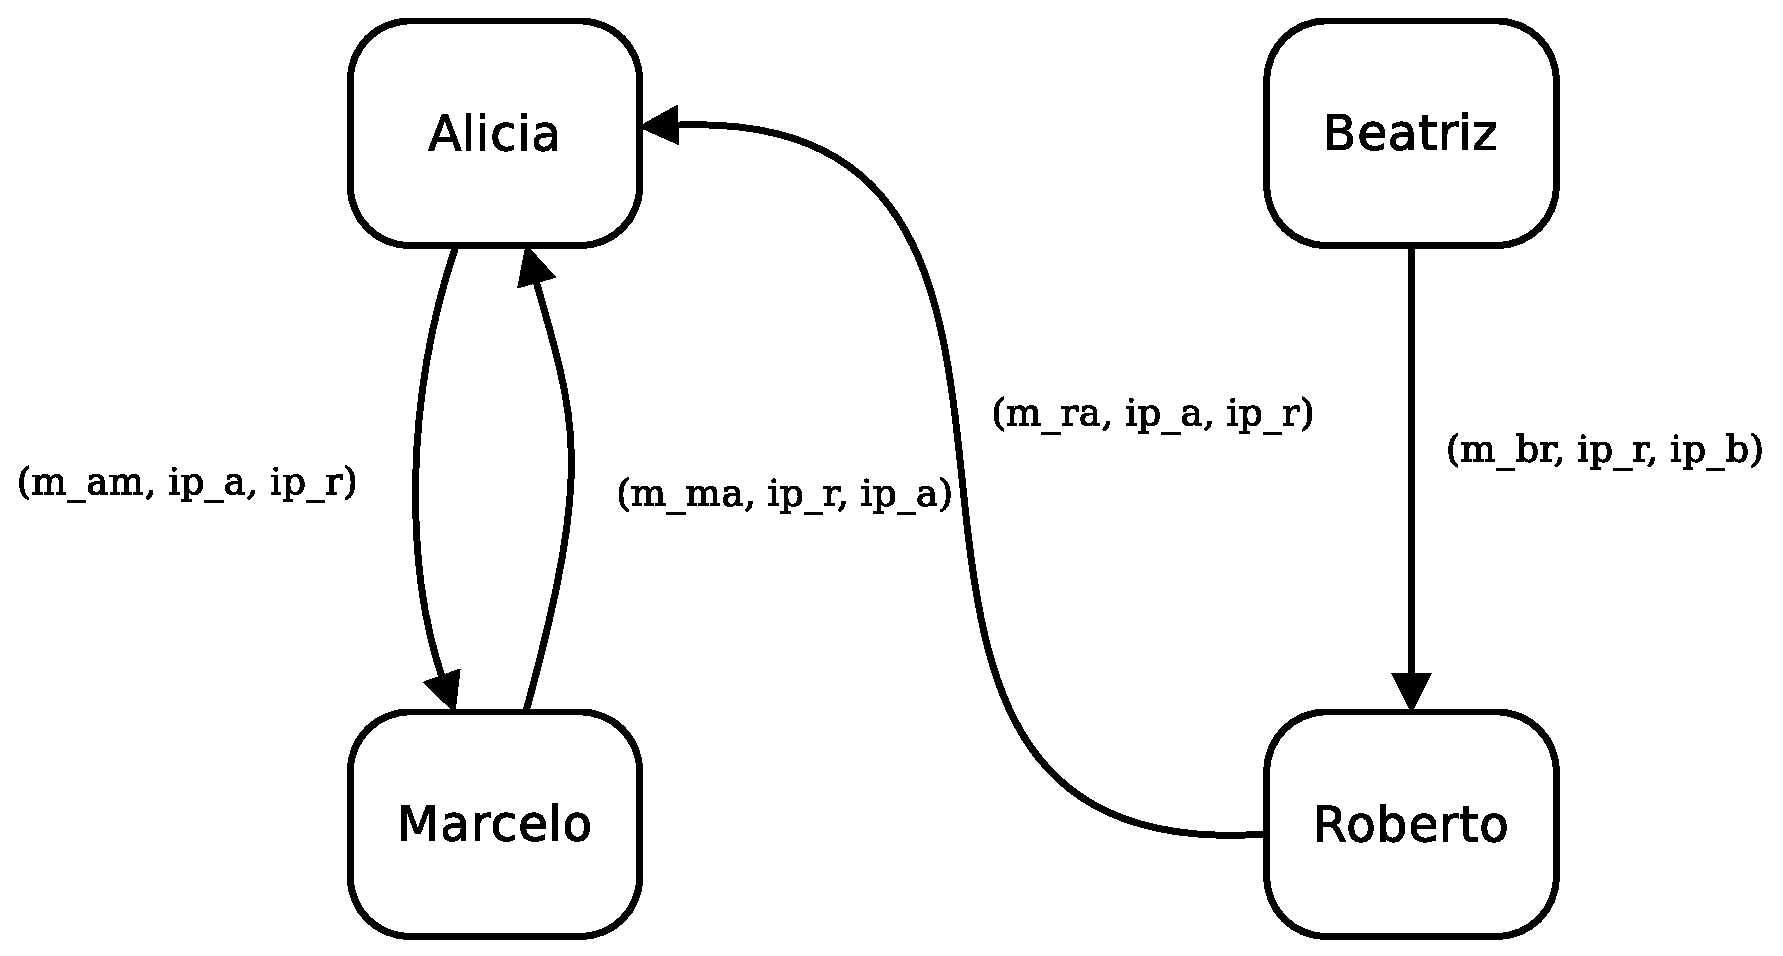
\includegraphics[width=0.7\textwidth]{figs/tcpip_simple}
    \caption{Protocolo simple de comunicación}
    \label{tcpip_simple}
\end{figure}

Para definir el anonimato resulta crucial definir formalmente que es considerado
un ataque al anonimato, pues un protocolo es anónimo si y solo si no existe ningún ataque.
En \cite{conf/pet/HeviaM08} se define un ataque con el siguiente juego.
El observador o adversario determinada dos posibles ejecuciones del protocolo, las cuales difieren en
qué mensajes son enviados por quién y qué mensajes son recibidos por quién. Entonces
consideraremos que el adversario realiza un ataque si al ejecutar al adversario con cada una
de las posibles ejecuciones del protocolo, el adversario logra identificar cuál es cuál.
Por lo tanto un protocolo sera seguro si y solo si cualquier adversario no logra distinguir
una ejecución de otra.

\subsubsection{Autentificación desmentible}
En el protocolo de la Figura \ref{tcpip_simple} es posible que un adversario (rol que puede
asumir una empresa $Empr-2$) se haga pasar por una empresa $Empr-1$ con buena reputación y denuncie
falsamente a una empresa enemiga $Empr-3$. Para ello
sólo es necesario que modifique uno de sus mensajes cambiando $ip_e2$ por $ip_e1$.
Por lo tanto decimos que el protocolo no implementa canales autentificados.\\
Con canales autentificados nos referimos protocolos en los cuales es posible estar seguro,
con alta probabilidad, de quién es el autor de un mensaje. Sin embargo hay que ser cuidadoso
con el protocolo de autentificación usado, pues los más conocidos
(firmas digitales por ejemplo) poseen la propiedad de \textit{non repudiability}. Esto es,
que el emisor de un mensaje autentificado no puede negar a ``la comunidad" que él es el autor
del mensaje. Esto estaría contradiciendo el anonimato, pues el adversario también sería capaz
de asociar la autoría de un mensaje a el emisor de éste.\\
La autentificación desmentible, introducida en \cite{DwoNaoSah04}, se refiere a los protocolos
que implementan canales anónimos con la propiedad adicional de que cada mensaje es autentificado
a un receptor específico y el receptor no es capaz de probar a nadie más quién es el autor del mensaje.

\subsubsection{Componibilidad}
En general, el hecho de implementar protocolos con ciertas garantías (por ejemplo ano\-ni\-ma\-to y
autentificación desmentible) no garantiza que dichas propiedades se sigan teniendo cuando
el protocolo es ejecutado concurrentemente con otros protocolos.\\
En \cite{conf/focs/Canetti01}, Canetti introduce el \textit{framework} criptográfico conocido
como \textit{Universal Composabillity} (desde ahora UC). UC propone una metodología para definir y
demostrar los objetivos de seguridad de un protocolo (por ejemplo anonimato y autentificación)
de un protocolo. UC garantiza que el protocolo mantiene su seguridad inclusive
si es ejecutado concurrentemente con cualquier protocolo, siempre y cuando no comparta estado
con el protocolo analizado.\\
Cuando el protocolo sí comparte estado con otros protocolo es necesario hacer uso del
\textit{framework Generalized Universal Composabillity} (desde ahora GUC), que generaliza a UC.
Informalmente GUC propone una metodología para incluir el estado que un protocolo podría compartir
con otros.

\section{Objetivos}

\subsection{Objetivo general}
Diseñar un protocolo criptográfico eficiente que cumpla nociones razonables
de Anonimato y Autentificación Desmentible. Demostrar matemáticamente su
seguridad usando herramientas modernas de análisis criptográficas (GUC) y
estudiar su relación con otras primitivas criptográficas.

\subsection{Objetivos específicos}

\begin{enumerate}
    \item Estudiar conceptos asociados a interacciones desmentibles y las técnicas y
          primitivas criptográficas asociadas (encriptación y mecanismos de autentificación
           como firmas digitales y esquemas de identificación).
    \item Estudiar conceptos de anonimato y las técnicas y primitivas criptográficas
          asociadas.
    \item Proponer un protocolo que combine ambas nociones.
    \item Analizar dicho protocolo en términos de efectividad y eficiencia.
    \item Analizar la efectividad en términos de las garantías de seguridad obtenidas.
    \item Analizar la eficiencia en términos de los costos en tiempo asociados al
          protocolo.
    \item Estudiar su relación con otros protocolos criptográficos.
\end{enumerate}


En la Figura \ref{sigmix_simple} se muestra un diagrama para explicar nuestra solución. A grandes
razgos, proponemos combinar un protocolo de autentificación desmentible con un protocolo de
canales anónimos. Es por ello que primero los mensajes enviados son procesados por el protcolo de
autentificación desmentible para luego ser distribuidos por el protocolo de canales anónimos.

\begin{figure}[hp]
    \centering
    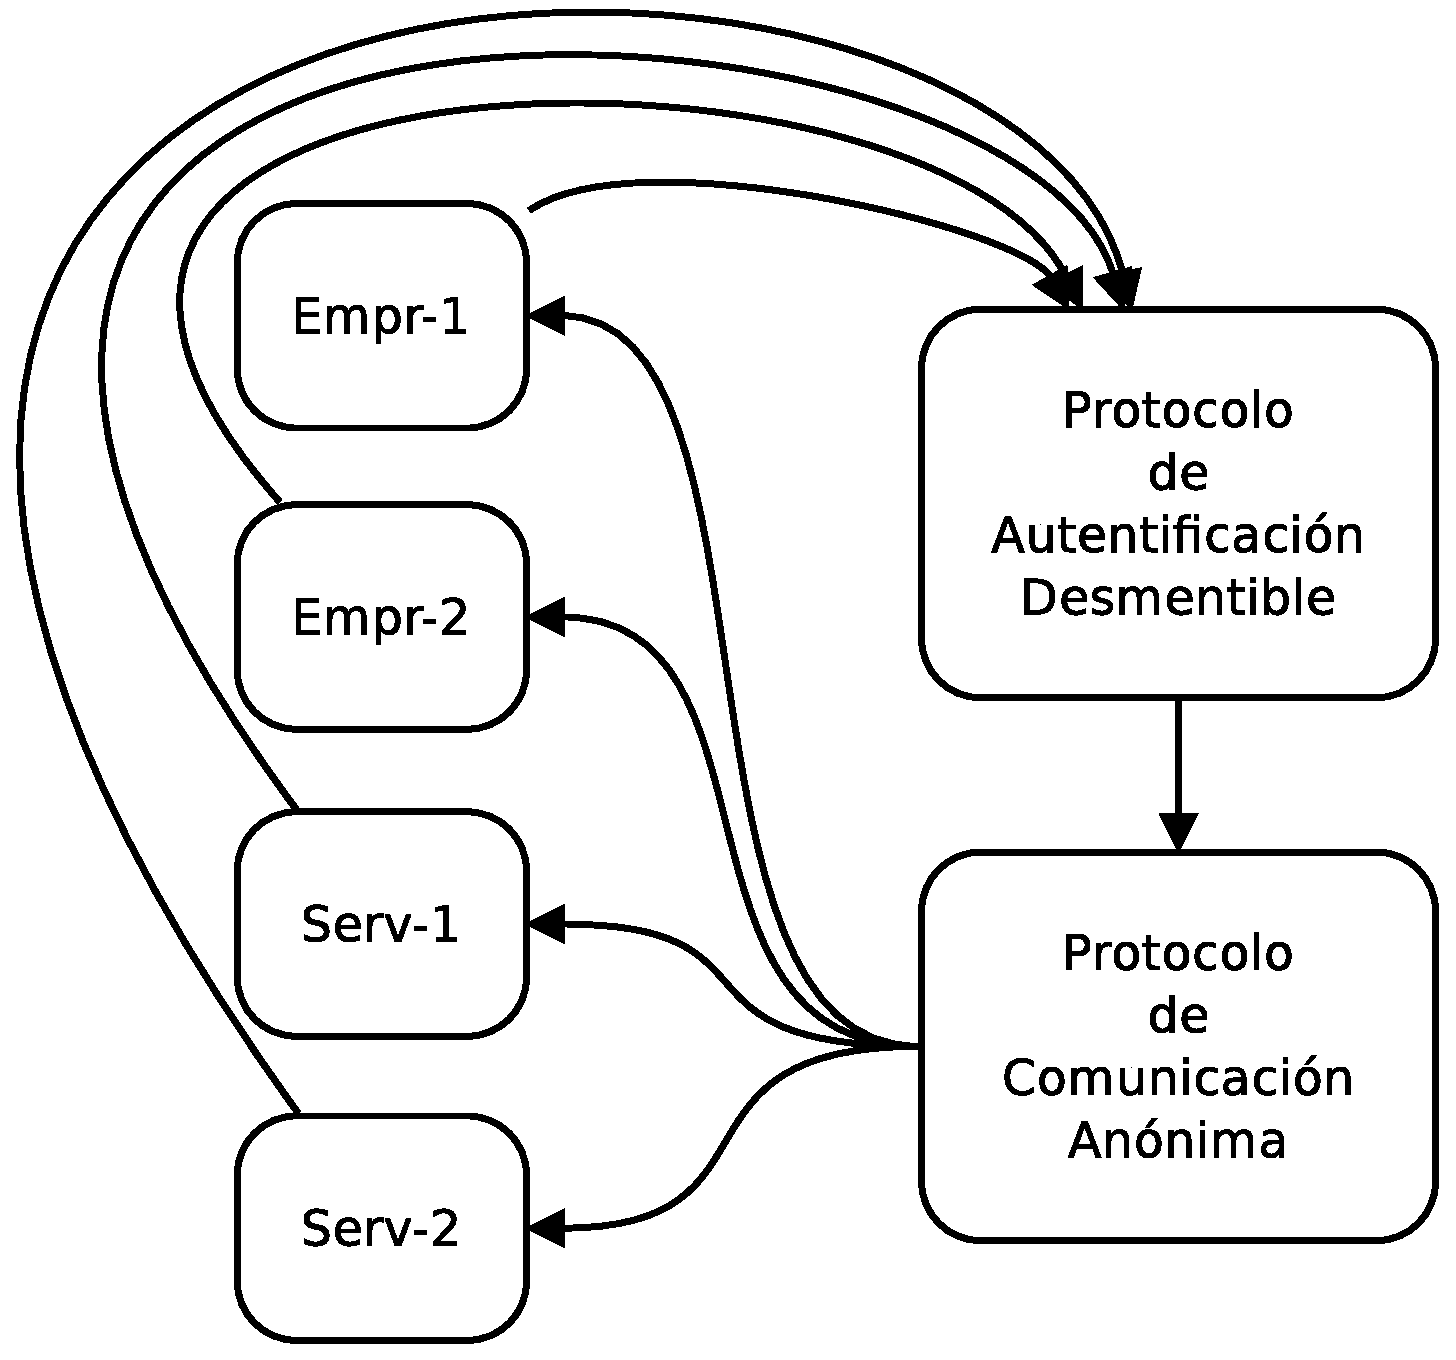
\includegraphics[width=0.5\textwidth]{figs/sigmix_simple}
    \caption{Solución propuesta}
    \label{sigmix_simple}
\end{figure}


%TODO Habrá un nombre mejor?
\chapter{Marco Teórico}

En este capítulos hacemos distintas definiciones básicas útiles
para este trabajo.

\section{Definiciones básicas}

\begin{definicion}[String]
Decimos que $\omega$ es un string si $\omega \in \{0,1\}^*$.
\end{definicion}

\begin{definicion}[Largo de un string]
Para un string $\omega$ denotamos por $|\omega|$ al entero $k$
talque $k$ es el número de caracteres de $|\omega|$.
\end{definicion}

\begin{definicion}[Función despreciable]
Decimos que una función $\eta: \mathbb{N} \to \mathbb{N}$ es despreciables
si crece más lento que el inverso de cualquier polinomio. Es decir, para
todo polinomio $p$ existe
un $n_0$ talque para todo $n > n_0$ se cumple que
$$\eta(n) < \frac{1}{p(n)}$$
\end{definicion}
Las funciones despreciables permiten definir probabilidades ``pequeñas'' cualquier
variable aleatorias ``algorítmicas'' (es decir corresponden a las salida de un algoritmo).
La definición busca eliminar el efecto de ejecutar una cantidad polinomial de veces un
algoritmo (usar el lema de amplificación).

\begin{definicion}[Grupo Abeliano]
Decimos que el par $(G,+)$, donde $G$ es un conjunto y
$+:G^2 \to G$, es un grupo abeliano si se cumplen las siguientes propiedades:
\begin{enumerate}
\item (Asocioatividad) $\forall a,b,c \in G$ $(a+b)+c=a+(b+c)$.
\item (Elemento neutro) $\exists 0 \in G$ talque $\forall a \in G$ $a+0 = 0+a = a$.
\item (Inverso) $\forall a \in G$ $\exists -a \in G$ talque $a+-a = 0$.
\item (Conmutatividad) $\forall a,b \in G$ $a+b = b+a$.
\end{enumerate}
\end{definicion}

En general cuando decimos que $G$ es un grupo nos referimos a que es un grupo abeliano.

\begin{definicion}[Generador]
Decimos que $g\in G$ es un generador de $G$ si el conjunto generado por $g$ 
$\langle g \rangle = \{g^n|n\in\mathbb{N}\}$ es igual a $G$
\end{definicion}

\begin{definicion}[Grupo cíclico]
Decimos que $G_q$ es un grupo cíclico de orden $q$ si existe un generador
$g$ de $G$ y $|G| = q$.

\end{definicion}

\section{Probabilidades discretas}

\begin{definicion}[Espacio de probabilidades finito]
Una espacio de probabilidades finito es un conjunto finito
$\Omega = \{\omega_1, \ldots, \omega_{|\Omega|}\}$ con un conjunto
de números $p_1, \ldots, p_{|\Omega|} \in [0,1]$ tales que
$\sum_{i=1}^{|\Omega|}p_i=1$
\end{definicion}

A menos que se especifique lo contrario, asumimos que la distribución
de $\Omega$ es uniforme, es decir $p_i = \frac{1}{|\Omega|}$. Al experimento
de escoger un $\omega$ en $\Omega$ al azar denotamos por $\omega \in_R \Omega$.

\begin{definicion}[Evento]
Decimos que $A$ es un evento de $\Omega$ si $A \subseteq \Omega$. Denotamos
por $\Pr[A] = \sum_{\omega_i \in A}p_i$  a la probabilidad de $A$
\end{definicion}

\begin{definicion}[Variable aleatoria]
Una variable aleatoria es una función $X:\Omega \to \mathbb{R}$ que asigna a
cada $\omega \in \Omega$ un número real $x \in \mathbb{R}$.
\end{definicion}

\begin{definicion}[Distribución]
Dada una varibale aleatoria, definimos su distribución como la función
$f:\mathbb{R} \to [0,1]$ talque $f(x) = \sum_{i:X(\omega_i)=x}p_i$
\end{definicion}

\begin{definicion}[Distancia estadística]
Dadas dos variables aleatoria $X$ e $Y$ definidas sobre $\Omega$, definimos
la distancia estadística entre ellas como
$$\Delta(X, Y) = \max_{S\subseteq \Omega}\{X(S)-Y(S)\}$$
\end{definicion}

\subsection{Indistinguibilidad}
La noción de indistinguibilidad es una noción fundamental en criptografía
pues ha permitido definir la seguridad mediante la similitud entre distintos
eventos.\\
La indistinguibilidad es una noción
de similaridad entre familias de variables aleatorias (o conjuntos
de variables aleatorias) y existen tres tipos de indistinguibilidad.

\begin{definicion}[Indistinguibilidad perfecta]
Decimos que dos familias de variables aleatorias $U=\{U_x\}_{x\in\{0,1\}^*}$
y $V=\{V_x\}_{x\in\{0,1\}^*}$ son perfectamente indistinguibles
si $\Delta(U_x, V_x)) = 0 \qquad \forall x$.
Denotamos la indistinguibilidad perfecta por escribimos $U_x = V_x$
\end{definicion}

\begin{definicion}[Indistinguibilidad estadística]
Decimos que dos familias de variables aleatorias $U=\{U_x\}_{x\in\{0,1\}^*}$ y 
$V=\{V_x\}_{x\in\{0,1\}^*}$ son estadísticamente indistinguibles
si $\Delta(U_x, V_x)$ es despreciable en $|x|$. Denotamos la indistinguibilidad estadística
por $U \approx Y$.
\end{definicion}

\begin{definicion}[Indistinguibilidad computacional]
Decimos que dos familias de variables aleatorias $U=\{U_x\}_{x\in\{0,1\}^*}$ y
$V=\{V_x\}_{x\in\{0,1\}^*}$ son estadísticamente indistinguibles
para todo algoritmo polinomial aleatorizado $A$ existe una función despreciable
$\eta$ y un entero $n_0$ talque si $|x| > n_0$
$|\Pr[A(U_x)=1] - \Pr[A(V_x)=1]| \leq \eta(|x|)$. Denotamos la indistinguibilidad
computacional por $U \overset{c}{\approx} V$.
\end{definicion}

\section{Definiciones criptográficas básicas}

\subsection{El problema de Diffie-Hellman decisonal (DDH)}
El problema DDH \cite{diffie-hellman_me:1976a} es un problema que se considera
difícil, es decir se conjetura
que no existe un algoritmo polinomial que lo solucione, para ciertos
grupos. DDH es una herramienta fundamental en la Criptografía moderna pues
permite la construcción eficientes primitivas con una variada aplicabilidad.

\begin{definicion}[DDH]
Sea $G_q$ un grupo cíclo de orden $q$. Decimos que en $G_q$ se cumple DDH
si las variables aleatorias $(g^\alpha, g^\beta, g^\gamma) \overset{c}{\approx}
(g^\alpha, g^\beta, g^{\alpha \cdot \beta})$ dado que $\alpha, \beta, \gamma \in_R G_q$.
\end{definicion}

\subsection{Esquemas de Encriptación}
Decimos que $\mathcal{E} = (K, E, D)$, con conjunto de textos planos $M$ y conjunto de textos
cifrados $C$,es un esquema de encriptación simétrico si para todo
$r \in \{0, 1\}^\kappa$, dado $k = K(\kappa; r)$ , para todo $m\in M$ $D_k(E_k(m))=m$.

Decimos que $\mathcal{E} = (K, E, D)$, con conjunto de textos planos $M$ y conjunto de textos
cifrados $C$,es un esquema de encriptación asimétrico si para todo
$r \in \{0, 1\}^\kappa$, dado $(sk, pk) = K(\kappa; r)$ , para todo $m\in M$ $D_{sk}(E_{pk}(m))=m$.


\subsection{Indistinguibilidad bajo ataque de texto plano escogido (IND-CPA)}
Tabién conocida como \textit{seguridad semántica} es una definición de privacidad de un esquema
critográfico. Apunta a que un esquema de encriptación $\mathcal{E} = (K, E, D)$ es seguro si ningún atacante es capaz de
dinstinguir entre la encriptación de cualesqueir par de mensajes $m_1, m_2$.


\begin{definicion}[Experimento IND-CPA]
Definimos el experimento IND-CPA parametrizado por un aloritmo $\mathcal{A}$,
un esquema de encriptación $\mathcal{E}$, parametro de seguridad $\kappa$ y
un bit $b$, denotado por $\mathrm{EXP}^\mathrm{IND-CPA}_\mathcal{E}(\mathcal{A}, b)$,
como la variable aleatoria resultante de
ejecutar el experimento descrito en la figura \ref{fig:ind_cpa}
\end{definicion}


\begin{definicion}[Seguridad IND-CPA]
Decimos que un esquema de encriptación $\mathcal{E}$ es IND-CPA seguro si
$$\mathrm{EXP}^\mathrm{IND-CPA}_\mathcal{E}(\mathcal{A}, 1) \approx
\mathrm{EXP}^\mathrm{IND-CPA}_\mathcal{E}(\mathcal{A}, 0)$$
\end{definicion}

\begin{figure}
\begin{centering}
\framebox{\begin{minipage}[t]{1\columnwidth}
El experimento IND-CPA  ejecutado con adversario $\mathcal{A}$, esquema de encritación $\mathcal{E} = (K, E, D)$,
un bit $b \in\{0,1\}$ y parámetro de seguridad $\kappa$ procede como sigue:
\begin{enumerate}
    \item Escoger las clave del esquema, $k \overset{R}{\leftarrow} K(\kappa)$.
    \item Ejecutar al adversario $\mathcal{A}$ y cada vez que escriba $(m_1, m_2)$ retornale $E_k(m_b)$.
    \item Retornar lo que $\mathcal{A}$ retorne.
\end{enumerate}
\end{minipage}}
\end{centering}
\caption{El experimento IND-CPA}
\label{fig:ind_cpa}
\end{figure}


\subsection{Infalsificabilidad ante ataques de mensajes escogidos UF-CMA}
UF-CMA aplica a esquemas de firmas de mensajes (\textit{Message Authentication Code} o MAC). Un esquema de firmas
es UF-CMA si ningún adversario es capaz de falsificar la firma de un mensaje 

\subsection{Algunas \textit{Setup assumptions} comunes}
\subsubsection{String público aleatorio CRS}
\subsubsection{Interfaz de clave pública PKI}



\chapter{Modelo Criptográfico}

Demostraremos las garantías de seguridad de nuestro protocolo en el
\textit{framework Generalized Universal Composability} (GUC). GUC \cite{conf/tcc/CanettiDPW07}
es una generalizacion del \textit{framework Universal Composability}
\cite{conf/focs/Canetti01}. Ambos sirven para modelar protocolos criptgráficos concurrentes,
pero GUC adicionalmente modela protocolos concurrentes que comparten estado entre si.
Primero revisaremos el framework UC pues GUC se construye a partir de UC con pequeñas,
pero muy significativas, modificaciones.\\

\section{The Universal Composability framework (UC)}
UC es una metodología para modelar modularizadamente protocolos criptograficos que son ejecutados en redes
del ``mundo real" (por ejemplo internet). El espiritu de UC es diseñar un protocolo y luego abstraer la
seguridad que uno espera de él en un protocolo ideal, ejecutado en condiciones especiales que garantizan
su seguridad. Luego se debe demostrar que ejecutar el protcolo real y ejecutar el protocolo ideal es
escencialmente lo mismo, por lo tanto el protocolo real es tan seguro como el protocolo ideal.\\
Los protocolos reales son pueden ser ejecutados concurrentemente con muchos otros protocolos,
y tambien pueden ser ejecutados distribuidos entre varios participantes.
Como en el mundo real el protocolo puede ser monitoreado por terceros y algunos participantes pueden salirse
arbitrareamente del protocolo atentando con la seguridad. Todo el posible mal comoportamiento es ejecutado por una sola
máquina, el Adversario (real) $\mathcal{A}$. En una ejecución del protocolo el adversario puede espíar y
manipular todos los mensajes intercambiados, también puede manejar la distribución de mensajes a su antojo,
y además puede \textit{corromper} participantes del protocolo y ejecutar codigo arbitrario en ellos.\\
Por otro lado estan los protocolos ideales, llamados \textit{funcionalidades ideales} denotadas por 
$\mathcal{F}$. Las funcionlidades ideales son ejecutadas en un mundo ideal, donde es una entidad confiable
la encargada de ejecutar su código. En el mundo ideal existe un adversario ideal o \textit{simulador}
$\mathcal{S}$, pero este no puede espíar ni controlar la comunicación más de lo que la funcionalidad ideal
permite.\\
La configuración en la que el protocolo real es ejecutado con el adversario real es conocida como \textit{mundo
real}, y la configuración en que la funcionalidad ideal es ejecutada con el adversario ideal es conocida como
\textit{mundo ideal}. En ambos mundos la ejecución del protocolo concurrentemente con otros protocolos esta a cargo
de una máquina especial conocida como el ambiente y denotado por $\mathcal{Z}$. De este modo en UC los protocolos
pueden ser analizados aislados de resto del mundo. Para asegurarse que el protcolo real alcanza la seguridad deseada
se debe tener que para cualquier ejecución del protocolo en el mundo real y para cualquier estrategia adversarial
(esto es para todo ambiente y para todo adversario) existe una estrategia adversarial con recursos limitados (un
adversario ideal) que tiene el mismo efecto que la estrategia adversarial real (el ambiento no es capaz de percatarse
de ninguna diferencia entre la ejecución del protocolo real y el protocolo ideal).\\
Para definir formalmente las nocienes intuitivas descritas anteriormente es necesario introducir un modelo de
cálculo conocido como Máquinda de Turing Interactiva , más precisamente sitemas de ITM.

\subsection{Sistemas de Máquinas de Turing Interactivas}

Las Máquinas de Turing Interactivas corresponden a Máquinas de Turing con cintas especiales que pueden ser
escritas externamente. A dichas cintas las llamamos escribibles externamente (EW), y son de escritura única,
es decir, el cabezal siempre se mueve a la derecha.

\newtheorem{definicion}{Definición}

\begin{definicion}
Una Máquina de Turing Interactiva $M$ es una Máquina de Turing con las siguientes cintas:
\begin{enumerate}
    \item Una cinta EW de identidad.
    \item Una cinta EW del parámetro de seguridad.
    \item Una cinta EW de entrada.
    \item Una cinta EW de comunicación entrante.
    \item Una cinta EW de salidas de subrutinas.
    \item Una cinta de salida.
    \item Una cinta de bits aleatorios.
    \item Una cinta de activación, de lectura y escritura y de 1 bit de tamaño.
    \item Una cinta de lectura y escritura para trabajo. 
\end{enumerate}
\end{definicion}

La cinta de identidad contiene un string que representa la identidad de $M$, que se interpreta
como si estuviera compuesto por dos substrings: el identificadod de sesión (SID) y el identificador
de participante (PID). Identificamos a cada instancia de una ITM (ITI) por el par
$\mu = (\langle M \rangle, id)$, con $\langle M \rangle$ el código de $M$ y $id$ el contenido de la cinta
de identidad. En general omitimos los $\langle \rangle$ y con $M$ nos referimos tanto a la máquina como
al código.\\
La cinta del parámetro de seguridad contiene un string de la forma $1^k$, con $k$ el parámetro de seguridad 
\footnote{El parámetro de seguridad indica el nivel de seguridad en el cual se esta ejecutando
la máquina, y en general mientras crece se debería tener que la seguridad del protocolo ejecutado
con la máquina también crece.}.\\
La cinta de salida contendrá la salida de $M$ una vez que haya terminado.\\
La cinta de bits aleatorios contiene suficientes bits aleatorios para que $M$ pueda realizar sus cálculos.\\
La cinta de trabajo es la usual cinta de trabajo de las Máquinas de Turing.\\
La cinta de activación tiene el valor 0 si la $M$ no esta activada y 1 si lo esta. La secuencia de
configuraciones de una ejecución de $M$
\footnote{Una configuración corresponde a un objeto que determina completamente un instante
en la computación de una MT. Podemos ver la ejecuciónde una MT como una secuencía de configuraciones, donde la
primera configuración corresponde a la MT en su estado inicial y la(s) cinta(s) con la(s) entrada(s), y la
configuración final corresponde a la MT en un estado final.}
esta compuesta por subsecuencias en las
que en cada configuración la $M$ esta activada. A dichas subsecuencias se les conoce como \textit{secuencias
de activación}.\\
Las otras cintas toman importancia cuando $M$ es ejecutada ``conectada" con otras máquina
en un Sistema de ITMs.\\

\begin{definicion}
Un Sistema de ITMs $S$ viene dado por $S = (I, C)$, donde $I$ es la ITM inicial y $C$ es la función
de control $C:\{0,1\}^* \to \{0,1\}$.
\end{definicion}
Inicialmente la ITI $\mu_0 = (I, 0)$ es activada, el sITM terminará cuando $I$ termine y su
salida sera la salida lo que $I$ deje en su cinta de salida.\\
Una ITI $\mu = (M, id)$ puede escribir en una de las cintas de otra ITI $\mu' = (M', id')$, 
para ello es necesario que $\mu$ ejecute una instrucción
especial llamada \texttt{escritura-externa} y debe especificar la cinta en de $\mu'$ en la que quiere
escribir y los datos a escribir en esa cinta
\footnote{Formalmente podríamos decir que $M$ entra en un estado especial y en su cinta de
trabajo se encuentra un string $x$ que determina $\mu'$, la cinta objetivo y los datos a escribir
en la cinta objetivo}.
La semántica de la instrucción de \texttt{escritura-externa} es como sigue:\\

\begin{enumerate}
    \item Si la funciónde control $C$ aplicada a toda la secuencia de intrucciones \texttt{escritura-externa}
          que se han realizado hasta ahora retorna 0, entonces la instrucción es ignorada.
    \item Si $C$ retorna 1 pero no existe una ITI en el sITM $\mu'' = (M'', id'')$ talque $id''=id'$, se
          crea una nueva ITI con código $M'$ y con identidad $id'$. Para ello se crea una nueva ITM
          que en la cinta de identidad contiene $id'$, el la cinta del parámetro de sugirdad contiene $1^k$
          y en la cinta de bits aleatorios contiene suficientes bits aleatorios. A continuación se evalúa
          el punto siguiente.
    \item Si $C$ retorna 1 y existe una ITI en el sITM $\mu'' = (M'', id'')$ talque $id''=id'$:
    \begin{enumerate}
        \item Si la cinta objetivo de la intrucción era la cinta de comunicación entrante de $\mu'$, entonces
              los datos especificados son escritos en la cinta de comunicación entrante de $\mu''$ y $\mu''$
              es activada. Notemos que esto es hecho independiente de si el código de $\mu''$ es el mismo
              código especificado por $\mu$, con el fin de rescatar que una ITI no conoce el código de la
              ITI con que se comunica a través de escrituras en la cinta de comunicación entrante.
        \item Si la cinta objetivo era la cinta de entrada de $\mu'$ y $M' = M''$, entonces los datos
              especificados son escritos en la cinta de entrada de $\mu''$ y $\mu''$ es activada. En este caso
              la instrucción modela llamados a otras ITIs como subrutina, dentro de un entorno seguro ($\mu$
              conoce el código que esta ejecutando $\mu''$).
        \item Si la cinta objetivo es la cinta de salida de subrutina de $\mu'$, entonces los datos
              especificados son escritos en la cinta de salida de subrutina de $\mu''$. En este caso la
              instrucción modela el retorno de una llamada a subrutina, en que la subrutina no conoce
              el código de la ITI que la llamó.
    \end{enumerate}
\end{enumerate}

Ahora estamos listos para definir la ejecución de un protocolo en UC

\subsection{Ejecución de un protocolo}

\section{Generalized Universal Composabillity}

Before the GUC framework were proposed an alternative way
to model protocols sharing state in the UC framework was the use of JUC theorem, but this is not as general as
it only allows protocols sharing state among themselves. Instead the GUC framework models protocols sharing state with
unpredictable other protocols.\\


\chapter{Desmentibilidad}
La Desmentibilidad puede tener distintas acepciones, por ejemplo Encriptación
desmentible \cite{CanettiEtAl97}. Aquí nos referimos a la noción de Desmentibilidad asociada
a la Autentificación desmentible.\\
La Autentificación desmentible fue introducida por Dwork, Nahor y Sahai en \cite{DwoNaoSah04}.
Variadas modificaciones, generalizaciones e implementaciones han sido propuestas posteriormente,
como por ejemplo en \cite{journals/joc/RaimondoG09}. Aquí consideraremos y adaptaremos la definición
hecha por Dodis, Katz, Smith y Walfish en \cite{conf/tcc/DodisKSW09}, dado que esa definición
es la que aplica a una configuración concurrente y distribuida como la necesaria en este trabajo.\\
Intuitivamente decimos que un protocolo es desmentible si nadie puede probar a otro que una sesión
del protocolo, es decir un grupo específico de participantes con identidades públicas definidas,
se esta llevando a cabo o alguna vez se llevó a cabo. En \cite{conf/tcc/DodisKSW09} se muestra que
para el caso de la autentificación la desmentibilidad se puede obtener considerando un juez que
en forma \textit{online} debe decidir con quién esta hablando: un informante que esta observando
una sesión real del protocolo de autentificación, o un desinformante que no tiene acceso a la sesión
real del protocolo pero aún así quiere convencer al juez que la sesión se esta llevando a cabo.
El protocolo se dirá entonces que es un protocolo de autentificación desmentible online si
para todo juez y para todo informante existe un desinformante tal
que el juez no puede distinguir
si habla con el informante o el desinformante. En la versión completa de \cite{conf/tcc/DodisKSW09}
se demuestra se demuestra que esta noción es equivalente a GUC-realizar la funcionalidad ideal
$\mathcal{F}_{AUTH}$. Dodis y compañía señalan que en GUC un protocolo que realiza una funcionalidad
ideal $\mathcal{F}$ es tan desmentible como $\mathcal{F}$. La funcionalidad ideal $\mathcal{F}_{AUTH}$
es ``completamente simulable'', lo que significa que el protocolo puede ser simulado completamente sin
la participación de ningún participante de la sesión, luego la funcionalidad $\mathcal{F}_{AUTH}$
es desmentible.\\
De forma similar que en \cite{conf/tcc/DodisKSW09}, pero sin restringirnos a protocolos de autentificación,
definiremos la noción de desmentibilidad en línea o \textit{online}.

\section{Desmentibilidad online}

Consideraremos dos \textit{mundos}: el mundo real, donde el informante tiene acceso directo a una sesión
del protocolo analizado; y el mundo simulado, donde el desinformante no tiene acceso al protocolo.
Nos restringiremos a funcionalidades ideales, pues la desmentibilidad es una propiedad a ser chequeada en la
funcionalidad ideal.

\begin{definicion}[Mundo real]
Sea $\mathcal{F}$ una funcionalidad ideal que se ejecuta en el modo $\bar{\mathcal{G}}$-híbrido con participantes
$\tilde{P}_1, \ldots, \tilde{P}_n$, sea $\mathcal{D}$ el adversario \textit{dummy}, sea $\mathfrak{I}$ el
informante, $\mathcal{J}$ el juez y sea
$(V_\mathcal{F}, E_\mathcal{F}) =
\mathfrak{I}(
    \mathcal{H}(
        \mathcal{F},
        \mathcal{D},
        \tilde{P}_1,
        \ldots,
        \tilde{P}_n,
        \{\tilde{P_i}\}^{\bar{\mathcal{G}}}))$.
Definimos el mundo real como el grafo de ITMs $\mathfrak{R} = (V, E)$ donde:
$$V = \{\mathcal{J}, \bar{\mathcal{G}}\} \cup V_\mathcal{F}$$
$$E = \{(\mathcal{J}, \mathfrak{I})\} \cup E_\mathcal{F}$$
Denotamos por $\mathrm{Real}_{\mathcal{F}, \mathcal{J}, \mathfrak{I}}^{Den}$ a la variable aleatoria
que describe la salida de $\mathcal{J}$ al ejecutarse el grafo de ITMs $\mathfrak{R}$
\end{definicion}

\begin{definicion}[Mundo simulado]
Sea $\mathcal{F}$ una funcionalidad ideal que se ejecuta en el modo $\bar{\mathcal{G}}$-híbrido con participantes
$\tilde{P}_1, \ldots, \tilde{P}_n$, sea $\mathcal{D}$ el adversario \textit{dummy}, sea $\mathfrak{D}$ el
desinformante, $\mathcal{J}$ el juez.
Definimos el mundo simulado como el grafo de ITMs $\mathfrak{S} = (V, E)$ donde:
$$V = \{\mathcal{J}, \bar{\mathcal{G}}, \mathfrak{D}\}$$
$$E = \{(\mathcal{J}, \mathfrak{D}),
        (\mathcal{J}, \bar{\mathcal{G}}),
        (\mathfrak{D}, \bar{\mathcal{G}})\}$$
Denotamos por $\mathrm{Sim}_{\mathcal{F}, \mathcal{J}, \mathfrak{D}}^{Den}$ a la variable aleatoria
que describe la salida de $\mathcal{J}$ al ejecutarse el grafo de ITMs $\mathfrak{S}$
\end{definicion}

Definimos la desmentibilidad como la incapacidad del juez para distinguir entre una ejecución
real informada por el informante de la funcionalidad de una ejecución simulada por el desinformante.

\begin{definicion}[Desmentibilidad]
Decimos que una funcionalidad $\mathcal{F}$ es
desmentible si para todo juez $\mathcal{J}$ y todo informante
$\mathfrak{I}$ existe un desinformante $\mathfrak{D}$ talque:
$$\mathrm{Real}_{\mathcal{F}, \mathcal{J}, \mathfrak{I}}^{Den} \approx
\mathrm{Sim}_{\mathcal{F}, \mathcal{J}, \mathfrak{D}}^{Den}$$
\end{definicion}

Notamos que el experimento $\mathrm{Real}_{\mathcal{F}, \mathcal{J}, \mathfrak{I}}^{Den}$ es una transformación
sintáctica de la ejecución en UC de la funcionalidad ideal $\mathcal{F}$, como lo demuestra el siguiente teorema.

\begin{teorema}
Para toda funcionalidad $\mathcal{F}$ ejecutada en el modelo $\bar{\mathcal{G}}$-híbrido se tiene que para
todo juez $\mathcal{J}$ y todo informante $\mathfrak{I}$ existe un ambiente $\mathcal{Z}$ talque
$$\mathrm{Real}_{\mathcal{F}, \mathcal{J}, \mathfrak{I}}^{Den} \approx
\mathcal{Z}(\mathcal{H}(
        \mathcal{F},
        \mathcal{D},
        \tilde{P}_1,
        \ldots,
        \tilde{P}_n,
        \{\tilde{P}_i\}^{\bar{\mathcal{G}}}))
$$
y también para todo ambiente $\mathcal{Z}$ existe un juez $\mathcal{J}$ y un informante $\mathfrak{I}$
tales que

$$\mathrm{Real}_{\mathcal{F}, \mathcal{J}, \mathfrak{I}}^{Den} \approx
\mathcal{Z}(\mathcal{H}(
        \mathcal{F},
        \mathcal{D},
        \tilde{P}_1,
        \ldots,
        \tilde{P}_n,
        \{\tilde{P}_i\}^{\bar{\mathcal{G}}}))
$$

\label{teo:den}
\end{teorema}

\begin{proof}
\textit{(Teorema \ref{teo:den})}\\
En efecto, cualquier combinación juez-informante puede ser simulada por un ambiente $\mathcal{Z}$,
lo que prueba la segunda afirmación de teorema.\\
Si consideramos un informante $\mathfrak{I}$ que solo comunica al juez $\mathcal{J}$ con los participantes
y el adversario dummy $\mathcal{D}$, el juez $\mathcal{J}$ es capaz de simular internamente a cualquier
ambiente $\mathcal{Z}$
pues $\mathfrak{I}$ le provee una interfaz con vista idéntica a la vista de $\mathcal{Z}$. Lo que nos
permite probar la primera afirmación del teorema.
\end{proof}

Como corolario del teorema \ref{teo:den} tenemos el siguiente resultado
\begin{corolario}
Sea $\pi$ protocolo que GUC-emula a una funcionalidad
ideal $\mathcal{F}$ desmentible. Entonces $\pi$ es desmentible.
\label{cor:den}
\end{corolario}

\begin{proof}
La demostración es directa dado que el experimento real para $\pi$ es identico a ejecutarlo en GUC.
Como $\pi$ GUC-emula a $\mathcal{F}$ existe un simulador que simula a $\pi$ con $\mathcal{F}$, el cual
puede ser usado para simular $\pi$ con el desinformate que existe para $\mathcal{F}$.
\end{proof}

\chapter{Anonimato} \label{sect:AC}
% Para que quede mejor podria poner tu definicion de anonimato, pero consecuentemente deberia probar
% que la funcionalidad ideal F_aac cumple con una de las defs. Cosa que no he hecho
Anonymous channels allow users to exchange messages without revealing their identities. Several protocols
have been proposed in the literature for anonymous channels. The modern study of anonymous channels was
started in \cite{journals/cacm/Chaum81} with \textit{mix-nets}. In a mix-net protocol the vector of all
parties encrypted messages are sent trough a set of \textit{mixers}. Each mixer perform an operation on cyphertexts
(usually partial decryption or reencryption) and send a random permutation to the next mixer. Finally the
last mixer publish a permutation of the vector of parties messages. Several modifications have been proposed
to mix-nets since Chaum's seminal paper, increasing tolerance to dishonest parties, robustness and many other
desirable properties.\\
To realize our protocol we use the universal composable mix net proposed by Wikstr\"om in \cite{Wikstrom04a}.
Basically Wikstr\"om's mix net proceeds as follows:

\begin{enumerate}

\item Each sender $P_i$ waits for mixers public keys and computes the product public key.
      Then each encrypt his message under the product public key, publish the cyphertext
      to a bulletin board an prove in zero knowledge that it is a valid cyphertext.
\item Each mix net $M_j$ $j\in{1, \ldots, k}$ discards all the published cyphertexts that
      are not valid. Then, for $l = 1, \ldots, k$ if $l = j$ the mixer partially decrypt
      the list of cyphertexts obtained from the bulletin board, perform a randomly chosen
      permutation on the list of cyphertext, publish on the bulletin board and prove in
      zero knowledge that the published list is a random permutation of the previous list.
      If $l \neq j$ the mixer must check that the permutation published by the mixer $M_l$
      is a valid one. Finally lexicographically sort the final published list and output it.

\end{enumerate}

In \cite{Wikstrom04a} is shown that this protocol UC-realize the ideal functionality $\mathcal{F}_{MN}$,
defined in figure \ref{func:F_MN}, in the $\mathcal{F}_{KG}-hybrid$ model. 
% Podria ser bueno In the apendix we show that this protocol also GUC-realize con F_KG share


\begin{figure}
\begin{centering}
\framebox{\begin{minipage}[t]{1\columnwidth}
\center{The Ideal functionality $\mathcal{F}_{MN}$ running with mixers $M_{1}, \ldots, M_{k}$, senders
        $P_{1}, \ldots, P_{N}$, and ideal adversary $\mathcal{S}$}
\begin{enumerate}
    \item Initialize a list $L = \emptyset$, and sets $J_P = \emptyset$ and $J_M = \emptyset$.
    \item Suppose $(P_{i}, \mathtt{Send}, m_{i})$  $m_{i} \in G_q$ is received from $\mathcal{C_I}$.
          If $i\notin J_P$, set $J_P \leftarrow J_P \cup \{i\}$, and append $m_i$ to the list $L$. Then
          hand $(\mathcal{S}, P_i, \mathtt{Send})$ to $\mathcal{C_I}$.
    \item Suppose $(M_{j}, \mathtt{Run})$ is received from $\mathcal{C_I}$. Set
          $J_M \leftarrow J_M \cup \{j\}$. If $|J_M | \geq k/2$, then sort the list $L$ lexicographically
          to form a list $L'$, and hand
          $((\mathcal{S}, M_{j}, \mathtt{Output}, L'), \{M_l , \mathtt{Output}, L'\}_{l=1}^{k})$ to
          to $\mathcal{C_I}$. Otherwise, hand $\mathcal{C_I}$ the list $(\mathcal{S}, M_{j}, \mathtt{Run})$
\end{enumerate}
\end{minipage}}
\end{centering}
\caption{The functionality $\mathcal{F}_{MN}$}
\label{func:F_MN}
\end{figure}


\input{./capitulos/protocolo.tex}
\chapter{Conclusiones}

En este trabajo se planteó el problema de comunicación anónima autentificada y se
demostró constructivamente que existe un protocolo que resuelve dicho problema.
Para ello se estudiaron tópicos avanzados de Criptografía como UC, GUC, Anonimato,
Desmentibilidad y distintas primitivas criptográficas asociadas a dichos tópicos.
Se definieron rigurosamente las propiedades que debe tener un protocolo para
resolver el problema planteado.
Se desarrolló un protocolo para el cual se puede garantizar matemáticamente que
satisface las propiedades necesarias para resolver el problema inicial.
El protocolo desarrollado es eficiente, pues se construye a partir de un protocolo
que se sabe eficiente por la comunidad \cite{Wikstrom04a} y adicionalmente efectúa
una operación que es lineal en el número de participantes del protocolo.\\

\section{Preguntas abiertas}

Adicionalmente, del trabajo realizado se desprenden las siguientes preguntas que han
quedado abiertas, pues escapan a los alcances de este trabajo. Sin embargo 
su sola formulación debe ser considerada un resultado de este trabajo, pues
estas preguntas proponen interesantes líneas de investigación.

\subsection{Mixnet GUC-segura}
El protocolo SIGMIX se construye a partir de una mixnet que en \cite{Wikstrom04a}
se demuestra UC-segura. Sin embargo, dado que para poder UC-realizar la mixnet
es necesario ocupar una setup assumption $\mathcal{F}_{KG}$, es válido preguntarse
si el protocolo de \cite{Wikstrom04a} sigue siendo seguro cuando $\mathcal{F}_{KG}$
es una funcionalidad compartida. En caso negativo es necesario preguntarse si existe
algún protocolo seguro para una mixnet con la setup assumption $\mathcal{F}_{KG}$.
Finalmente, si todos los esfuerzos han fracasado es necesario preguntarse si existe
una setup assumption compartida razonable con la cual se pueda GUC-realizar una
mixnet.\\

\subsection{Una modelación más exacta de la componibilidad en GUC}
El objetivo principal de GUC era modelar protocolos que se pueden componer
concurrentemente con otros protocolos que posiblemente comparten estado y de los
cuales nada se puede asumir. Sin embargo en el trabajo de esta memoria nos dimos
cuenta de que en la literatura, para el caso de PKI y CRS,
\footnote{En este caso se hace uso de uno funcionalidad compartida más fuerte
que CRS conocida como \textit{Augmented Common Random String}}
\textbf{sí se hacen suposiciones sobre los protocolos con los cuales el protocolo
analizado} se componen.\\
Para caso de PKI se asume que los protocolos
que hacen uso de la funcionalidad ideal $\bar{\mathcal{G}}_{KRK}$ se encuentran
dentro de un conjunto de protocolos $\Phi$. En general general $\Phi$ solo
contiene al protocolo analizado, por lo que la situación puede resultar muy
similar a JUC.\\
El caso de CRS es algo distinto, pero se puede mostrar que es equivalente. En
efecto, a la funcionalidad ideal que modela CRS se le especifica que debe
distinguir entre los participantes honestos y no honestos. Si bien en
\cite{Walfish:2008:ESM:1467461} notan que asumir esto es irreal, afirman que en
la práctica los participantes deben tener cuidado con no revelar cierto valor
secreto. Lo anterior no es más que una limitación a los protocolos que puede
ejecutar cada participante, pues $\Phi$ correspondería a protocolo que no revelan
el valor antes mencionado.\\
Adicionalmente, que solo protocolos en un conjunto $\Phi$
pueden acceder a la funcionalidad compartida no es posible de formalizar en EUC.
Si bien es posible de formalizar en GUC, es posible pensar en un modelo más general
donde $\Phi$ no depende de propiedades estáticas de los protocolos si no que de
propiedades dinámicas. Lo anterior no es formalizable en GUC, y para ellos es necesario
hacer ciertas modificaciones a GUC


%%%%%%%%%%%%%%%%%%%%%%%%%%%%%%
\bibliographystyle{abbrv}
\bibliography{biblio}{}
%\begin{additional}
%\section{Ambiente de desarrollo}

%\section{Glosario}
%\section{Material Complementario}
%\end{additional}

\end{document}
